\documentclass{isma-thesis}

\usepackage[protrusion]{microtype}

% --- Algorithms (float + pseudocode)
\usepackage{algorithm}
\usepackage{algpseudocode}

% % --- Code listings with minted (creates a 'listing' float)
% \usepackage[newfloat]{minted} % compile with -shell-escape
% --- Code listings without external deps
\usepackage{listings}
\lstset{
  basicstyle=\ttfamily\small,
  numbers=left,
  numbersep=6pt,
  frame=single,
  breaklines=true,
  tabsize=2,
  float=htbp, % keep if you want floaty listings
  captionpos=t % caption on top (to match your template)
}
% Optional: pick a mono font explicitly
% \setmonofont{Mono} % or Consolas/DejaVu Sans Mono/etc.


% --- Bibliography via biblatex ---
\usepackage[backend=biber,style=ieee,sorting=nty,maxbibnames=99]{biblatex}
\addbibresource{x_bibliography/references.bib}

% ====== Fill these in (example placeholders) ======
\setthesisinfoLV
  {<BSC DARBA NOSAUKUMS ŠEIT>}% LV Title
  {Vārds Uzvārds}% LV Student
  {Dr. Prof. Vadītāja Vārds Uzvārds, PhD}% LV Supervisor
  {42484 Informācijas sistēmas (bak.)}% LV Study programme
  {Dabaszinātņu un datortehnoloģiju katedra}% LV Department
  {2025}% Year

\setthesisinfoEN
  {<BSC THESIS TITLE GOES HERE>}% EN Title
  {Name Surname}% EN Student
  {Dr. Prof. Supervisor Name Surname, PhD}% EN Supervisor
  {42484 Information Systems (BSc)}% EN Study programme
  {Department of Natural Sciences and Computer Engineering}% EN Department
  {2025}% Year

\begin{document}

% frontmatter/title_page_lv.tex
\thispagestyle{empty}

% --- Top-left wide logo ---
\noindent
\includegraphics[width=\rnulogowidth]{\rnulogopath}

\vspace{6mm}

% --- One line: left label, right programme ---
\begin{tabular*}{\textwidth}{@{}l@{\extracolsep{\fill}}r@{}}
  {\bfseries\fontsize{12pt}{12pt}\selectfont Studiju programma} &
  {\bfseries\fontsize{12pt}{12pt}\selectfont \studyprogrammeLV} \\
\end{tabular*}

\vspace{8mm}

% --- Centered department ---
\begin{center}
  {\bfseries\fontsize{16pt}{16pt}\selectfont \departmentLV}
\end{center}

\vspace{10mm}

% --- Main centered block: ISMA name + Title + work type + meta ---
\begin{center}
  {\Large RĪGAS ZIEMEĻVALSTU UNIVERSITĀTE}\\[2mm]
  {\Large (RNU)}\\[8mm]

  {\bfseries\fontsize{16pt}{16pt}\selectfont \thesistitleLV}\\[10mm]
  {\bfseries\large BAKALAURA DARBS}\\[18mm]

  \begin{tabular}{@{}p{6cm}p{8cm}@{}}
    Students:& \studentnameLV\\[2mm]
    Darba vadītājs:& \supervisornameLV\\
  \end{tabular}

  \vfill
  {\thesiscityLV\ \thesisyear}
\end{center}


\clearpage
\thispagestyle{empty}

\noindent
\includegraphics[width=\ismalogowidth]{\ismalogopath}

\vspace{6mm}

\noindent
\begin{tabular*}{\textwidth}{@{}l@{\extracolsep{\fill}}r@{}}
  {\bfseries\fontsize{12pt}{12pt}\selectfont Study Programme} &
  {\bfseries\fontsize{12pt}{12pt}\selectfont \studyprogrammeEN} \\
\end{tabular*}

\vspace{8mm}

\begin{center}
  {\bfseries\fontsize{16pt}{16pt}\selectfont \departmentEN}
\end{center}

\vspace{10mm}

\begin{center}
  {\Large INFORMATION SYSTEMS MANAGEMENT INSTITUTE}\\[2mm]
  {\Large (ISMA)}\\[8mm]

  {\bfseries\fontsize{16pt}{16pt}\selectfont \thesistitleEN}\\[10mm]
  {\bfseries\large BACHELOR'S THESIS}\\[18mm]

  \begin{tabular}{@{}p{6cm}p{8cm}@{}}
    Student:& \studentnameEN\\[2mm]
    Supervisor:& \supervisornameEN\\
  \end{tabular}

  \vfill
  {\thesiscityEN\ \thesisyear}
\end{center}

\clearpage

% Page numbering starts at Title page but number not printed there (done).
% Show numbers from here:
\pagenumbering{arabic}

% ===== Abstracts & Keywords =====
\frontmatterpage
\unchapter{Anotācija}
Bakalaura darba mērķis ir pasākumu izstrāde personāla motivācijas sistēmas uzņēmumā “X” pilnveidošanai, lai mazinātu personāla mainību un ar to saistītās izmaksas. Darbs sastāv no ievada, četrām daļām, secinājumiem, literatūras saraksta un pielikumiem.

Pirmajā daļā analizētas teorētiskās pieejas personāla motivācijas sistēmas izpētei.
Otrajā daļā sniegta uzņēmuma “X” darbības vispārīga analīze.
Trešajā daļā veikts uzņēmuma “X” personāla motivācijas sistēmas pētījums.
Ceturtajā daļā piedāvāti priekšlikumi motivācijas sistēmas pilnveidei un tās ekonomiskās efektivitātes novērtējums.

Metodiskā bāze: zinātniskā literatūra, statistikas dati un uzņēmuma “X” iekšējā dokumentācija; izmantotas salīdzinošās analīzes, statistikas un aptaujas metodes.

\textbf{Atslēgvārdi:} personāls, personāla vadība, personāla motivācija, motivācijas sistēma, materiālā motivācija, nemateriālā motivācija, izmaksas.

\frontmatterpage
\unchapter{Abstract}
The main aim of the Bachelor Paper is to develop measures to improve the employee motivation system at Enterprise X in order to reduce personnel turnover and related costs. The Paper consists of the introduction, four parts, conclusions, references, and appendices.

Part one reviews theoretical approaches to employee motivation systems.
Part two presents a general analysis of Enterprise X.
Part three studies the current employee motivation system at Enterprise X.
Part four proposes improvements and evaluates their economic efficiency.

Methods: comparative analysis of scientific literature, analysis of primary and secondary statistics, internal documentation review, and a survey study.

\textbf{Key words:} personnel, personnel management, employee motivation, motivation system, material motivation, non-material motivation, costs.

\frontmatterpage
\unchapter{Key words / Atslēgvārdi}
\begin{tabular}{p{0.45\linewidth}p{0.45\linewidth}}
\textbf{Personnel} & \textbf{Personāls}\\
Personnel management & Personāla pārvalde\\
Employee motivation & Personāla motivācija\\
Employee motivation system & Personāla motivācijas sistēma\\
Material motivation & Materiālā motivācija\\
Non-material motivation & Nemateriālā motivācija\\
Costs & Izmaksas\\
\end{tabular}
\clearpage


% ===== Table of Contents (and optional lists) =====
\tableofcontents

% ---- Meta lists: each on its own page, and not added to ToC ----
\clearpage
\begingroup\let\addcontentsline\relax\listoffigures\endgroup

\clearpage
\begingroup\let\addcontentsline\relax\listoftables\endgroup

\clearpage
\begingroup\let\addcontentsline\relax\listofalgorithms\endgroup

\clearpage
% \begingroup\let\addcontentsline\relax\listoflistings\endgroup
\begingroup\let\addcontentsline\relax\lstlistoflistings\endgroup
\clearpage



% ===== Chapters =====
% Unnumbered Introduction (still added to ToC)
\unchapter{Introduction}
The problem of employee motivation is driven by instability and staff reduction across many sectors. Under these conditions, enterprises face the task of retaining qualified personnel—thus improving the motivation system becomes essential.

\textbf{Aim of the study:} to develop measures to improve the employee motivation system at Enterprise X.

\textbf{Object of the study:} the entrepreneurial activity of Enterprise X.

\textbf{Subject of the study:} the employee motivation system at Enterprise X.

\textbf{Problem:} high personnel turnover which increases enterprise costs.

\textbf{Tasks:}
\begin{enumerate}
  \item Review theoretical approaches to employee motivation systems.
  \item Provide a general analysis of Enterprise X.
  \item Study the current employee motivation system at Enterprise X.
  \item Develop improvement measures and evaluate their economic efficiency.
\end{enumerate}

\textbf{Hypothesis:} implementing the proposed measures will improve service quality and reduce turnover.

\textbf{Research methods:} survey methods, theoretical analysis, inductive/deductive reasoning, statistical and graphical methods.

\textbf{Approbation of the study (if any):} list presentations, publications, and expert reviews here.


\chapter{Theoretical approaches to the study of employee motivation}
\section{Concept of employee motivation}
Provide definitions and literature review; end with brief sub-conclusions.

\section{Basic theories of employee motivation}
Compare classic and contemporary theories; outline implications.

\section{System approach to employee motivation}
\subsection{Principles of employee motivation}
\subsection{Types of employee motivation}

\noindent\textbf{Conclusions (for Chapter 1).} Brief paragraph summarizing the main theoretical takeaways.

% ---- Figure example (title under figure; centered) ----
\begin{figure}[h]
  \centering
  
\includegraphics[width=0.7\linewidth]{b_chapters/chapter1/assets/isma_logo.png}
  \caption{Example grouped illustration of motivation drivers}
  \label{fig:motivation-drivers}
\end{figure}

% ---- Table example (title above; single spacing) ----
{\singlespacing
\begin{table}[h]
  \caption{Research results (example)}
  \label{tab:research-results}
  \centering
  \begin{tabular}{lrrrr}
    \toprule
    Factor & A & B & C & D\\
    \midrule
    Pay & 2 & 23 & 23 & 3\\
    Recognition & 4 & 18 & 19 & 2\\
    Growth & 5 & 21 & 16 & 4\\
    \bottomrule
  \end{tabular}

  \vspace{2mm}
  \emph{Source:} author’s calculation based on data from Enterprise X.
\end{table}
}

\chapter{Case / System Analysis (Example Chapter~2)}
\label{chap:analysis}

% --- IMPORTANT NOTE FOR STUDENTS ---
% This is only a suggested structure and sample content.
% You are free to modify, reorder, merge, or rename sections
% if it makes sense for your topic — as long as your supervisor agrees.

This chapter often provides a structured analysis of the case, dataset, or system that your thesis investigates.  
However, its scope and layout depend heavily on the chosen topic. Some theses merge this part into the empirical chapter; others expand it into multiple chapters.  
Think of the following sections as \emph{examples}, not as mandatory rules.

\section{General Characteristics of the Case / System (Example Section)}
\label{sec:case}
Here you may describe the case or system under study (e.g., an IT application, dataset, algorithm, protocol, or infrastructure).  
Mention background, design, stakeholders, or technical architecture.  

\paragraph{Note.} Adapt the level of detail to your project.  
If your work is purely theoretical, this section can be shorter. If it is applied to a concrete system or dataset, give enough context so the reader understands what is being studied.

\section{Analysis of Internal and External Environment (Optional Example)}
\label{sec:env}
Depending on your topic, you might include a structured breakdown of the system.  
Possible angles include (choose those that fit, or invent your own):

\begin{itemize}[leftmargin=1.2cm]
  \item \textbf{Architecture.} Components, modules, services, or data pipelines.
  \item \textbf{Performance.} Scalability, latency, throughput, bottlenecks.
  \item \textbf{Security and reliability.} Threats, vulnerabilities, resilience.
  \item \textbf{External factors.} Standards, APIs, dependencies, regulations.
\end{itemize}

Support your analysis with diagrams, tables, or references if relevant.

% --- Example figure (replace or remove) ---
\begin{figure}[h]
  \centering
  
\includegraphics[width=0.65\linewidth]{b_chapters/chapter1/assets/RNU_large_logo.png}
  \figsource{Replace with your own system diagram (if needed).}
  \caption{Example system architecture diagram.}
  \label{fig:analysis-example}
\end{figure}

% --- Example table (replace or remove) ---
{\singlespacing
\begin{table}[h]
  \caption{Example system metrics (dummy data)}
  \label{tab:analysis-example}
  \centering
  \begin{tabular}{lrr}
    \toprule
    Metric & Baseline value & Target value \\
    \midrule
    Response time (ms)  & 240   & 120   \\
    Uptime (\%)         & 97.5  & 99.9  \\
    Requests / second   & 350   & 1000  \\
    \bottomrule
  \end{tabular}
\end{table}
}

\section{Context, Constraints, and Risks (Optional)}
\label{sec:constraints}
In some topics, it is useful to state the limitations and boundary conditions that affect your system. Examples:

\begin{itemize}[leftmargin=1.2cm]
  \item Technical constraints (hardware, data availability, standards compliance).
  \item Research constraints (time, scope, access rights).
  \item Risks (privacy, security, reliability, scalability challenges).
\end{itemize}

This subsection can be skipped if not relevant.

\section{Data and Methods for the Analysis (Example)}
\label{sec:datamethods}
Briefly outline what data and methods you are using here.  
Examples: logs, benchmark datasets, architectural specifications, monitoring tools.  
Methods could include profiling, simulation, descriptive statistics, or qualitative inspection.  
Adapt this to your project; the goal is only to show that your analysis has a methodological basis.

\section{Sub-Conclusions (for Chapter~2)}
\label{sec:subconcl}
End with a short synthesis (typically 1–3 paragraphs).  
Example points to cover:

\begin{itemize}[leftmargin=1.2cm]
  \item What the analysis revealed (main technical insights).
  \item Which constraints/risks are most critical for your research.
  \item How this motivates the next step (empirical study in Chapter~\ref{chap:empirical}).
\end{itemize}

\paragraph{Reminder.} This subsection is not meant to repeat the whole chapter — just connect the dots and prepare for the next one.


\chapter{Empirical Study / Practical Research (Example Chapter~3)}
\label{chap:empirical}

% --- Guidelines for students ---
% Chapter 3 is often the empirical or applied part of the thesis:
% - field survey, experiments, prototype, modelling, case study, etc.
% The size and contents depend on your topic.
% Remember: quality and clarity are more important than length.

\section{Design of the Study}
Describe how your empirical work was set up: objectives, participants/subjects, instruments/tools, sampling method, procedures.

\section{Results of the Study}
Present your results in a structured way (tables, figures, text). Explain what you observed. Do not interpret too much here (save in Chapter 4 “Discussion”).

% Example: small figure with dummy data
\begin{figure}[h]
  \centering
  
\includegraphics[width=0.6\linewidth]{b_chapters/chapter1/assets/isma_logo.png}
  \figsource{Replace with your own chart or diagram.}
  \caption{Example chart of study results.}
  \label{fig:study-results}
\end{figure}

\section{Sub-Conclusions (for Chapter~3)}
Briefly summarize the main empirical findings (2–3 paragraphs). Link them back to the aim and hypothesis, but keep the deeper discussion for the next chapter.

% --- Note ---
% If your thesis only has 2 chapters, merge Chapters 2 and 3 into one.
% If you need more space (e.g., empirical + evaluation), you may split
% into 3 or even 4 chapters. Adjust flexibly.
\chapter{Development of the improved employee motivation system}
\section{Proposals for improvement}
Describe measures: material and non-material; implementation plan.

\section{Evaluation of economic efficiency}
Assumptions, cost-benefit, sensitivity analysis.

\noindent\textbf{Conclusions (for Chapter 4).} What works best and why.

\chapter{Discussion, Limitations, and Future Work (Optional Example Chapter~5)}
\label{chap:optional-discussion}

% --- IMPORTANT NOTE FOR STUDENTS ---
% This chapter is fully optional.
% Your thesis is complete without it, as long as you have a proper Conclusions chapter.
% Use it only if you feel that broader reflection or forward-looking remarks
% add significant value to your work (and your supervisor approves).

This chapter is meant as an *extra space* for broader reflection.  
It can be useful if you want to go beyond the mandatory Conclusions and show awareness of the bigger picture.  
However, it should remain concise and focused — do not just repeat results already covered in previous chapters.

\section{Extended Discussion (Optional)}
\label{sec:extended-discussion}
Here you may reflect on your findings in greater depth.  
Examples of what to include:

\begin{itemize}[leftmargin=1.2cm]
  \item Compare your results to other studies or real-world applications.  
  \item Highlight unexpected outcomes or open questions.  
  \item Discuss theoretical or practical implications that extend beyond your specific project.  
\end{itemize}

\paragraph{Tip.} This section can be especially valuable if your work connects to ongoing research, industrial practice, or societal issues.

\section{Limitations of the Study (Optional)}
\label{sec:limitations}
Every project has constraints — being open about them increases credibility.  
Possible categories:

\begin{itemize}[leftmargin=1.2cm]
  \item \textbf{Scope.} Narrow focus, specific use case, or limited generalizability.  
  \item \textbf{Data/technical.} Small datasets, noisy logs, hardware/software constraints.  
  \item \textbf{Methodological.} Simplifying assumptions, lack of longitudinal data, limited metrics.  
\end{itemize}

\paragraph{Note.} Do not exaggerate — just acknowledge realistically what was and wasn’t possible within your timeframe and resources.

\section{Future Work and Recommendations (Optional)}
\label{sec:future}
Suggest what could be done after your thesis.  
Examples:

\begin{itemize}[leftmargin=1.2cm]
  \item Follow-up studies or new research questions raised by your findings.  
  \item Practical improvements to your system, prototype, or methods.  
  \item Opportunities for scaling up, applying to other domains, or testing with different datasets.  
\end{itemize}

This section is not required, but it can demonstrate initiative and forward thinking.

\section*{Final Note}
\label{sec:finalnote}
Remember: the \textbf{mandatory Conclusions chapter} must already confirm the research tasks, validate the hypothesis, and state whether the aim of the thesis has been achieved.  
This optional chapter is only for broader reflection and forward-looking remarks — use it only if it adds real value.


% ===== Conclusions =====
\chapter{Conclusions}

The \textbf{Conclusions} chapter must clearly demonstrate that the aim and tasks of the Bachelor Paper have been fulfilled. This chapter is not a repetition of earlier text, but a synthesized summary that links the research aim, tasks, hypothesis, and results.

When preparing this section, students should ensure that:

\begin{itemize}
  \item \textbf{Confirmation of tasks.} Explicitly state that all tasks set out in the Introduction have been completed. A good practice is to connect each task with the chapter where it was accomplished.  
  Example:  
  “Task 1 (literature review) was completed in Chapter 1, providing a theoretical framework for the study. Task 2 (analysis of the case/system) was carried out in Chapter 2. Task 3 (empirical study) was presented in Chapter 3. Task 4 (development of proposals) was fulfilled in Chapter 4.”
  
  \item \textbf{Validation of hypothesis.} Clearly indicate whether the research hypothesis (if formulated) was validated or rejected, based on the obtained results.  
  Example:  
  “The proposed hypothesis was confirmed, as the empirical results demonstrated …”
  
  \item \textbf{Achievement of the aim.} Explicitly state that the aim of the thesis has been reached, supported by the fact that all tasks were accomplished and the hypothesis was addressed.  
  Example:  
  “Therefore, it can be concluded that the aim of the thesis has been achieved.”
  
  \item \textbf{Avoid repetition.} Do not copy entire findings from chapters. Instead, summarize them concisely to show the logical progression from tasks → results → aim.
  
  \item \textbf{Practical and theoretical value.} Conclude with a short statement on the significance of the results (e.g., how the findings may be used in practice or contribute to the field).
\end{itemize}

\noindent
\textbf{Recommended final formulation:}  
“All tasks set out in the Introduction were accomplished (Tasks 1–4 correspond to Chapters 1–4). The research hypothesis was validated, and the aim of the thesis has been reached.”


% ===== Literature =====
\printbibliography[heading=bibintoc,title=Literature]


% ===== Appendices =====
\appendix
\chapter{Appendix A — LaTeX Hints}
\label{chap:latexhints}


\newenvironment{twocoldemo}[1][]{%
  \par\noindent
  \begin{minipage}[t]{.48\linewidth}\raggedright
  \textbf{Code}\par\smallskip
}{%
  \end{minipage}\hfill
  \begin{minipage}[t]{.48\linewidth}\raggedright
  \textbf{Output}\par\smallskip
  \end{minipage}\par
}



This appendix shows small, copy-pasteable examples that compile with this thesis class out of the box. It avoids any template-specific commands from other classes.

\section{Paragraphs and inline emphasis}
Write one sentence per source line (helps with version control). A blank line starts a new paragraph.

You can write \emph{emphasized (italics)} and \textbf{bold} text. Use \verb|\url{...}| for clickable links, e.g.\ \url{https://ctan.org}.

\section{Math and equations}
Inline math: $f(x)=x^2+1$. Numbered display equations use \texttt{amsmath}:
\begin{align}
  \label{eq:sample}
  \int_0^1 x^2\,dx = \frac{1}{3}.
\end{align}
We can reference \cref{eq:sample} thanks to \texttt{cleveref}.

\section{Figures and subfigures}
A normal figure:
\begin{figure}[h]
  \centering
  
\includegraphics[width=.7\linewidth]{b_chapters/chapter1/assets/isma_logo.png}
  \caption{Example figure.}
  \label{fig:example}
\end{figure}

Two images side-by-side via \texttt{subcaption}:
\begin{figure}[h]
  \centering
  \begin{subfigure}{.47\linewidth}
    \centering
    
\includegraphics[width=.9\linewidth]{b_chapters/chapter1/assets/isma_logo.png}
    \caption{Left}
    \label{fig:left}
  \end{subfigure}\hfill
  \begin{subfigure}{.47\linewidth}
    \centering
    
\includegraphics[width=.9\linewidth]{b_chapters/chapter1/assets/isma_logo.png}
    \caption{Right}
    \label{fig:right}
  \end{subfigure}
  \caption{Two subfigures.}
  \label{fig:two-subfigs}
\end{figure}

We can reference \cref{fig:example,fig:two-subfigs,fig:left}.

\section{Tables}
A compact table with \texttt{booktabs}:
\begin{table}[h]
  \caption{Compact example table}
  \label{tab:compact}
  \centering
  \begin{tabular}{lrr}
    \toprule
    Factor & Mean & SD\\
    \midrule
    Pay           & 2.0 & 0.5\\
    Recognition   & 4.0 & 0.7\\
    Growth        & 5.0 & 0.6\\
    \bottomrule
  \end{tabular}
\end{table}

A long table across multiple pages (\texttt{longtable}):
\begin{longtable}{llr}
\caption{Long table example}\label{tab:long}\\
\toprule
\textbf{Item} & \textbf{Group} & \textbf{Value}\\
\midrule
\endfirsthead
\toprule
\textbf{Item} & \textbf{Group} & \textbf{Value}\\
\midrule
\endhead
\bottomrule
\endfoot
A & Alpha & 1\\
B & Alpha & 2\\
C & Beta  & 3\\
A & Alpha & 1\\
B & Alpha & 2\\
C & Beta  & 3\\
A & Alpha & 1\\
B & Alpha & 2\\
C & Beta  & 3\\
A & Alpha & 1\\
B & Alpha & 2\\
C & Beta  & 3\\
A & Alpha & 1\\
B & Alpha & 2\\
C & Beta  & 3\\
A & Alpha & 1\\
B & Alpha & 2\\
C & Beta  & 3\\
A & Alpha & 1\\
B & Alpha & 2\\
C & Beta  & 3\\
A & Alpha & 1\\
B & Alpha & 2\\
C & Beta  & 3\\
A & Alpha & 1\\
B & Alpha & 2\\
C & Beta  & 3\\
A & Alpha & 1\\
B & Alpha & 2\\
C & Beta  & 3\\
A & Alpha & 1\\
B & Alpha & 2\\
C & Beta  & 3\\
\end{longtable}

A landscape figure page (\texttt{pdflscape}):
\begin{landscape}
\begin{figure}[h]
  \centering
  
\includegraphics[width=.9\linewidth]{b_chapters/chapter1/assets/isma_logo.png}
  \caption{Landscape example.}
\end{figure}
\end{landscape}

\section{Algorithms and code listings}
Pseudocode with \texttt{algorithm}+\texttt{algpseudocode}:
\begin{algorithm}[h]
\caption{Greedy selection (example)}
\begin{algorithmic}[1]
  \State Initialize $S \gets \emptyset$
  \While{feasible choice exists}
    \State choose best feasible item $x$
    \State $S \gets S \cup \{x\}$
  \EndWhile
  \State \Return $S$
\end{algorithmic}
\label{alg:greedy-app}
\end{algorithm}

Code with \texttt{listings}:
% \begin{lstlisting}[language=Python,caption={Bubble sort},label={lst:bubble-app}]
% def bubble(a):
%     n = len(a)
%     for i in range(n-1):
%         for j in range(n-1-i):
%             if a[j] > a[j+1]:
%                 a[j], a[j+1] = a[j+1], a[j]
% \end{lstlisting}
{\captionsetup{type=lstlisting}
\begin{lstlisting}[language=Python,caption={Bubble sort},label={lst:bubble-app}]
def bubble(a):
    n = len(a)
    for i in range(n-1):
        for j in range(n-1-i):
            if a[j] > a[j+1]:
                a[j], a[j+1] = a[j+1], a[j]
\end{lstlisting}
}



We can reference \cref{alg:greedy-app,lst:bubble-app}.

\section{TikZ and (optional) pgfplots}
A tiny TikZ graphic:
\begin{figure}[h]
  \centering
  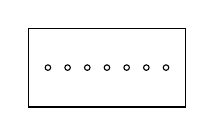
\begin{tikzpicture}
    \draw (0,0) rectangle (2,1);
    \foreach \x in {0.25,0.5,...,1.75} \draw (\x,0.5) circle (1pt);
  \end{tikzpicture}
  \caption{Simple TikZ demo.}
\end{figure}

If \texttt{pgfplots} is installed (we auto-load it if present), a quick plot:
\IfFileExists{pgfplots.sty}{%
\begin{figure}[h]
  \centering
  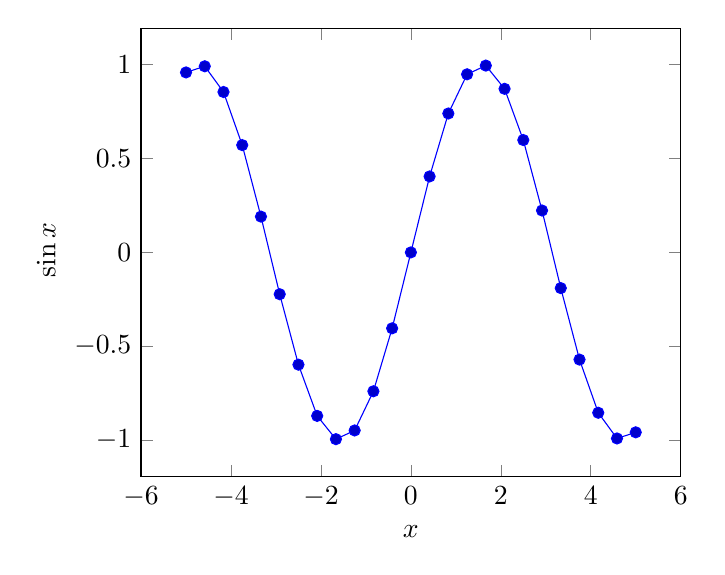
\begin{tikzpicture}
    \begin{axis}[xlabel=$x$,ylabel={$\,\sin x$}]
      \addplot {sin(deg(x))};
    \end{axis}
  \end{tikzpicture}
  \caption{Sine plot with pgfplots.}
\end{figure}
}{\noindent\emph{(pgfplots not installed — skipping plot.)}}

\section{Cross-references}
Use \verb|\label{...}| and \verb|\cref{...}| for equations, figures, tables, algorithms, and listings to get correct names and numbers automatically.

\section{Bibliography citation}
Cite like \cite{porter2008} and list all sources in the “Literature” section (managed by \texttt{biblatex} with the IEEE style in this project).

% ===== Declarations & Acknowledgments (if needed at end) =====
\frontmatterpage
\unchapter{Apliecinājums / Affirmation}
\textit{Ar šo es, \studentnameLV, apliecinu, ka bakalaura darbs ir izpildīts patstāvīgi, bez citu palīdzības, no svešiem avotiem ņemtie dati un definējumi ir uzrādīti darbā. Šis darbs nekādā veidā nav iesniegts nevienai citai pārbaudījuma komisijai un nekur nav publicēts.}

\vspace{12mm}
\noindent \textit{(Hereby I, \studentnameEN, affirm that the Bachelor's thesis was performed independently; sources of data and definitions are provided. This work has not been submitted to any other examination commission and has not been published elsewhere.)}

\vspace{14mm}
\noindent Rīga, 20\underline{\hspace{1cm}}.\ \underline{\hspace{2.5cm}}.\hspace{1cm}\rule{5cm}{0.4pt}\\
\hspace*{7.1cm}\scriptsize paraksts/signature, atšifrējums/decription \hfill

\frontmatterpage
\unchapter{Pateicības / Acknowledgments}
Autors izsaka pateicību darba vadītājam par sniegtajiem padomiem un atbalstu, kā arī uzņēmuma “X” kolēģiem par palīdzību datu iegūšanā un aptaujas realizēšanā.

The authors express gratitude to their supervisor for the provided advice and support, as well as to the colleagues at "X" company for their assistance in data acquisition and the implementation of the survey.

\end{document}
